\documentclass[1p]{elsarticle_modified}
%\bibliographystyle{elsarticle-num}

%\usepackage[colorlinks]{hyperref}
%\usepackage{abbrmath_seonhwa} %\Abb, \Ascr, \Acal ,\Abf, \Afrak
\usepackage{amsfonts}
\usepackage{amssymb}
\usepackage{amsmath}
\usepackage{amsthm}
\usepackage{scalefnt}
\usepackage{amsbsy}
\usepackage{kotex}
\usepackage{caption}
\usepackage{subfig}
\usepackage{color}
\usepackage{graphicx}
\usepackage{xcolor} %% white, black, red, green, blue, cyan, magenta, yellow
\usepackage{float}
\usepackage{setspace}
\usepackage{hyperref}

\usepackage{tikz}
\usetikzlibrary{arrows}

\usepackage{multirow}
\usepackage{array} % fixed length table
\usepackage{hhline}

%%%%%%%%%%%%%%%%%%%%%
\makeatletter
\renewcommand*\env@matrix[1][\arraystretch]{%
	\edef\arraystretch{#1}%
	\hskip -\arraycolsep
	\let\@ifnextchar\new@ifnextchar
	\array{*\c@MaxMatrixCols c}}
\makeatother %https://tex.stackexchange.com/questions/14071/how-can-i-increase-the-line-spacing-in-a-matrix
%%%%%%%%%%%%%%%

\usepackage[normalem]{ulem}

\newcommand{\msout}[1]{\ifmmode\text{\sout{\ensuremath{#1}}}\else\sout{#1}\fi}
%SOURCE: \msout is \stkout macro in https://tex.stackexchange.com/questions/20609/strikeout-in-math-mode

\newcommand{\cancel}[1]{
	\ifmmode
	{\color{red}\msout{#1}}
	\else
	{\color{red}\sout{#1}}
	\fi
}

\newcommand{\add}[1]{
	{\color{blue}\uwave{#1}}
}

\newcommand{\replace}[2]{
	\ifmmode
	{\color{red}\msout{#1}}{\color{blue}\uwave{#2}}
	\else
	{\color{red}\sout{#1}}{\color{blue}\uwave{#2}}
	\fi
}

\newcommand{\Sol}{\mathcal{S}} %segment
\newcommand{\D}{D} %diagram
\newcommand{\A}{\mathcal{A}} %arc


%%%%%%%%%%%%%%%%%%%%%%%%%%%%%5 test

\def\sl{\operatorname{\textup{SL}}(2,\Cbb)}
\def\psl{\operatorname{\textup{PSL}}(2,\Cbb)}
\def\quan{\mkern 1mu \triangleright \mkern 1mu}

\theoremstyle{definition}
\newtheorem{thm}{Theorem}[section]
\newtheorem{prop}[thm]{Proposition}
\newtheorem{lem}[thm]{Lemma}
\newtheorem{ques}[thm]{Question}
\newtheorem{cor}[thm]{Corollary}
\newtheorem{defn}[thm]{Definition}
\newtheorem{exam}[thm]{Example}
\newtheorem{rmk}[thm]{Remark}
\newtheorem{alg}[thm]{Algorithm}

\newcommand{\I}{\sqrt{-1}}
\begin{document}

%\begin{frontmatter}
%
%\title{Boundary parabolic representations of knots up to 8 crossings}
%
%%% Group authors per affiliation:
%\author{Yunhi Cho} 
%\address{Department of Mathematics, University of Seoul, Seoul, Korea}
%\ead{yhcho@uos.ac.kr}
%
%
%\author{Seonhwa Kim} %\fnref{s_kim}}
%\address{Center for Geometry and Physics, Institute for Basic Science, Pohang, 37673, Korea}
%\ead{ryeona17@ibs.re.kr}
%
%\author{Hyuk Kim}
%\address{Department of Mathematical Sciences, Seoul National University, Seoul 08826, Korea}
%\ead{hyukkim@snu.ac.kr}
%
%\author{Seokbeom Yoon}
%\address{Department of Mathematical Sciences, Seoul National University, Seoul, 08826,  Korea}
%\ead{sbyoon15@snu.ac.kr}
%
%\begin{abstract}
%We find all boundary parabolic representation of knots up to 8 crossings.
%
%\end{abstract}
%\begin{keyword}
%    \MSC[2010] 57M25 
%\end{keyword}
%
%\end{frontmatter}

%\linenumbers
%\tableofcontents
%
\newcommand\colored[1]{\textcolor{white}{\rule[-0.35ex]{0.8em}{1.4ex}}\kern-0.8em\color{red} #1}%
%\newcommand\colored[1]{\textcolor{white}{ #1}\kern-2.17ex	\textcolor{white}{ #1}\kern-1.81ex	\textcolor{white}{ #1}\kern-2.15ex\color{red}#1	}

{\Large $\underline{12n_{0044}~(K12n_{0044})}$}

\setlength{\tabcolsep}{10pt}
\renewcommand{\arraystretch}{1.6}
\vspace{1cm}\begin{tabular}{m{100pt}>{\centering\arraybackslash}m{274pt}}
\multirow{5}{120pt}{
	\centering
	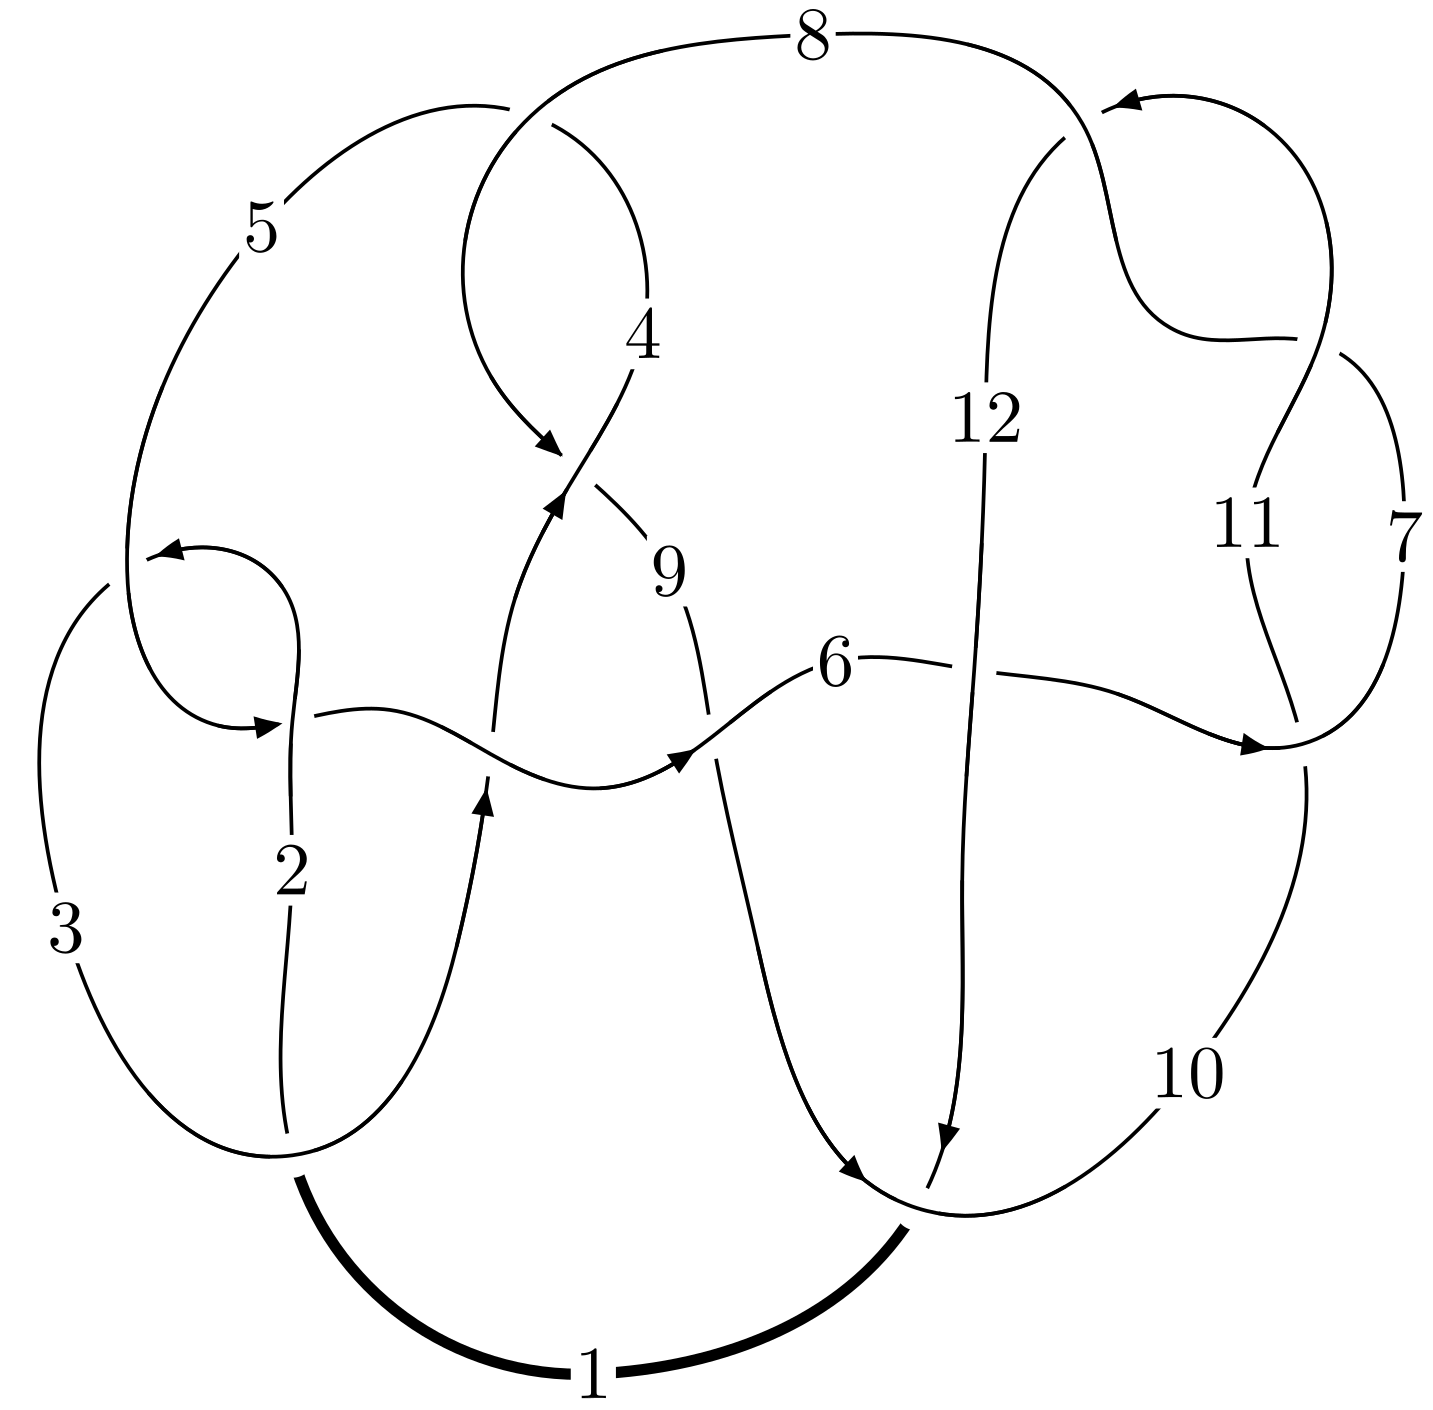
\includegraphics[width=112pt]{../../../GIT/diagram.site/Diagrams/png/2133_12n_0044.png}\\
\ \ \ A knot diagram\footnotemark}&
\allowdisplaybreaks
\textbf{Linearized knot diagam} \\
\cline{2-2}
 &
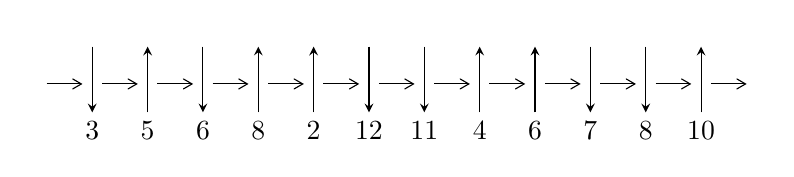
\begin{tikzpicture}[x=20pt, y=17pt]
	% nodes
	\node (C0) at (0, 0) {};
	\node (C1) at (1, 0) {};
	\node (C1U) at (1, +1) {};
	\node (C1D) at (1, -1) {3};

	\node (C2) at (2, 0) {};
	\node (C2U) at (2, +1) {};
	\node (C2D) at (2, -1) {5};

	\node (C3) at (3, 0) {};
	\node (C3U) at (3, +1) {};
	\node (C3D) at (3, -1) {6};

	\node (C4) at (4, 0) {};
	\node (C4U) at (4, +1) {};
	\node (C4D) at (4, -1) {8};

	\node (C5) at (5, 0) {};
	\node (C5U) at (5, +1) {};
	\node (C5D) at (5, -1) {2};

	\node (C6) at (6, 0) {};
	\node (C6U) at (6, +1) {};
	\node (C6D) at (6, -1) {12};

	\node (C7) at (7, 0) {};
	\node (C7U) at (7, +1) {};
	\node (C7D) at (7, -1) {11};

	\node (C8) at (8, 0) {};
	\node (C8U) at (8, +1) {};
	\node (C8D) at (8, -1) {4};

	\node (C9) at (9, 0) {};
	\node (C9U) at (9, +1) {};
	\node (C9D) at (9, -1) {6};

	\node (C10) at (10, 0) {};
	\node (C10U) at (10, +1) {};
	\node (C10D) at (10, -1) {7};

	\node (C11) at (11, 0) {};
	\node (C11U) at (11, +1) {};
	\node (C11D) at (11, -1) {8};

	\node (C12) at (12, 0) {};
	\node (C12U) at (12, +1) {};
	\node (C12D) at (12, -1) {10};
	\node (C13) at (13, 0) {};

	% arrows
	\draw[->,>={angle 60}]
	(C0) edge (C1) (C1) edge (C2) (C2) edge (C3) (C3) edge (C4) (C4) edge (C5) (C5) edge (C6) (C6) edge (C7) (C7) edge (C8) (C8) edge (C9) (C9) edge (C10) (C10) edge (C11) (C11) edge (C12) (C12) edge (C13) ;	\draw[->,>=stealth]
	(C1U) edge (C1D) (C2D) edge (C2U) (C3U) edge (C3D) (C4D) edge (C4U) (C5D) edge (C5U) (C6U) edge (C6D) (C7U) edge (C7D) (C8D) edge (C8U) (C9D) edge (C9U) (C10U) edge (C10D) (C11U) edge (C11D) (C12D) edge (C12U) ;
	\end{tikzpicture} \\
\hhline{~~} \\& 
\textbf{Solving Sequence} \\ \cline{2-2} 
 &
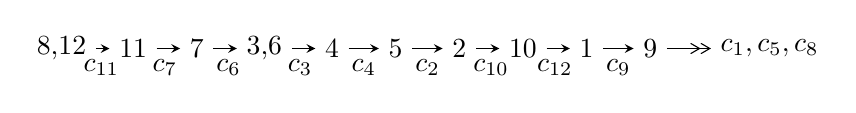
\begin{tikzpicture}[x=23pt, y=7pt]
	% node
	\node (A0) at (-1/8, 0) {8,12};
	\node (A1) at (1, 0) {11};
	\node (A2) at (2, 0) {7};
	\node (A3) at (49/16, 0) {3,6};
	\node (A4) at (33/8, 0) {4};
	\node (A5) at (41/8, 0) {5};
	\node (A6) at (49/8, 0) {2};
	\node (A7) at (57/8, 0) {10};
	\node (A8) at (65/8, 0) {1};
	\node (A9) at (73/8, 0) {9};
	\node (C1) at (1/2, -1) {$c_{11}$};
	\node (C2) at (3/2, -1) {$c_{7}$};
	\node (C3) at (5/2, -1) {$c_{6}$};
	\node (C4) at (29/8, -1) {$c_{3}$};
	\node (C5) at (37/8, -1) {$c_{4}$};
	\node (C6) at (45/8, -1) {$c_{2}$};
	\node (C7) at (53/8, -1) {$c_{10}$};
	\node (C8) at (61/8, -1) {$c_{12}$};
	\node (C9) at (69/8, -1) {$c_{9}$};
	\node (A10) at (11, 0) {$c_{1},c_{5},c_{8}$};

	% edge
	\draw[->,>=stealth]	
	(A0) edge (A1) (A1) edge (A2) (A2) edge (A3) (A3) edge (A4) (A4) edge (A5) (A5) edge (A6) (A6) edge (A7) (A7) edge (A8) (A8) edge (A9) ;
	\draw[->>,>={angle 60}]	
	(A9) edge (A10);
\end{tikzpicture} \\ 

\end{tabular} \\

\footnotetext{
The image of knot diagram is generated by the software ``\textbf{Draw programme}" developed by Andrew Bartholomew(\url{http://www.layer8.co.uk/maths/draw/index.htm\#Running-draw}), where we modified some parts for our purpose(\url{https://github.com/CATsTAILs/LinksPainter}).
}\phantom \\ \newline 
\centering \textbf{Ideals for irreducible components\footnotemark of $X_{\text{par}}$} 
 
\begin{align*}
I^u_{1}&=\langle 
2 u^{34}+4 u^{33}+\cdots+2 b-3 u,\;-6 u^{34}-12 u^{33}+\cdots+2 a-5,\;u^{35}+3 u^{34}+\cdots- u+1\rangle \\
I^u_{2}&=\langle 
u^3 a- a u+b- a,\;- u^3 a- u^4+u^3+a^2+2 a u+2 u^2-2 u-1,\;u^5- u^4-2 u^3+u^2+u+1\rangle \\
\\
\end{align*}
\raggedright * 2 irreducible components of $\dim_{\mathbb{C}}=0$, with total 45 representations.\\
\footnotetext{All coefficients of polynomials are rational numbers. But the coefficients are sometimes approximated in decimal forms when there is not enough margin.}
\newpage
\renewcommand{\arraystretch}{1}
\centering \section*{I. $I^u_{1}= \langle 2 u^{34}+4 u^{33}+\cdots+2 b-3 u,\;-6 u^{34}-12 u^{33}+\cdots+2 a-5,\;u^{35}+3 u^{34}+\cdots- u+1 \rangle$}
\flushleft \textbf{(i) Arc colorings}\\
\begin{tabular}{m{7pt} m{180pt} m{7pt} m{180pt} }
\flushright $a_{8}=$&$\begin{pmatrix}0\\u\end{pmatrix}$ \\
\flushright $a_{12}=$&$\begin{pmatrix}1\\0\end{pmatrix}$ \\
\flushright $a_{11}=$&$\begin{pmatrix}1\\- u^2\end{pmatrix}$ \\
\flushright $a_{7}=$&$\begin{pmatrix}u\\- u^3+u\end{pmatrix}$ \\
\flushright $a_{3}=$&$\begin{pmatrix}3 u^{34}+6 u^{33}+\cdots-\frac{3}{2} u+\frac{5}{2}\\- u^{34}-2 u^{33}+\cdots-\frac{7}{2} u^2+\frac{3}{2} u\end{pmatrix}$ \\
\flushright $a_{6}=$&$\begin{pmatrix}- u^3+2 u\\- u^3+u\end{pmatrix}$ \\
\flushright $a_{4}=$&$\begin{pmatrix}u^{34}+2 u^{33}+\cdots- u+1\\-2 u^{34}-\frac{7}{2} u^{33}+\cdots+u-\frac{1}{2}\end{pmatrix}$ \\
\flushright $a_{5}=$&$\begin{pmatrix}u^{34}+2 u^{33}+\cdots- u+1\\-4 u^{34}-\frac{13}{2} u^{33}+\cdots+3 u-\frac{3}{2}\end{pmatrix}$ \\
\flushright $a_{2}=$&$\begin{pmatrix}u^{34}+2 u^{33}+\cdots-\frac{5}{2} u+\frac{1}{2}\\\frac{1}{2} u^{32}+\frac{1}{2} u^{31}+\cdots+\frac{7}{2} u^2+\frac{3}{2} u\end{pmatrix}$ \\
\flushright $a_{10}=$&$\begin{pmatrix}- u^2+1\\u^4-2 u^2\end{pmatrix}$ \\
\flushright $a_{1}=$&$\begin{pmatrix}u^6-3 u^4+2 u^2+1\\- u^8+4 u^6-4 u^4\end{pmatrix}$ \\
\flushright $a_{9}=$&$\begin{pmatrix}- u^{10}+5 u^8-8 u^6+3 u^4+u^2+1\\- u^{10}+4 u^8-5 u^6+2 u^4- u^2\end{pmatrix}$\\&\end{tabular}
\flushleft \textbf{(ii) Obstruction class $= -1$}\\~\\
\flushleft \textbf{(iii) Cusp Shapes $= \frac{13}{2} u^{34}+\frac{21}{2} u^{33}+\cdots-15 u+\frac{21}{2}$}\\~\\
\newpage\renewcommand{\arraystretch}{1}
\flushleft \textbf{(iv) u-Polynomials at the component}\newline \\
\begin{tabular}{m{50pt}|m{274pt}}
Crossings & \hspace{64pt}u-Polynomials at each crossing \\
\hline $$\begin{aligned}c_{1}\end{aligned}$$&$\begin{aligned}
&u^{35}+24 u^{34}+\cdots-4 u-1
\end{aligned}$\\
\hline $$\begin{aligned}c_{2},c_{5}\end{aligned}$$&$\begin{aligned}
&u^{35}+6 u^{34}+\cdots-8 u-1
\end{aligned}$\\
\hline $$\begin{aligned}c_{3}\end{aligned}$$&$\begin{aligned}
&u^{35}-6 u^{34}+\cdots+u-2
\end{aligned}$\\
\hline $$\begin{aligned}c_{4},c_{8}\end{aligned}$$&$\begin{aligned}
&u^{35}- u^{34}+\cdots+2048 u+1024
\end{aligned}$\\
\hline $$\begin{aligned}c_{6}\end{aligned}$$&$\begin{aligned}
&u^{35}-9 u^{34}+\cdots+959 u-176
\end{aligned}$\\
\hline $$\begin{aligned}c_{7},c_{10},c_{11}\end{aligned}$$&$\begin{aligned}
&u^{35}+3 u^{34}+\cdots- u+1
\end{aligned}$\\
\hline $$\begin{aligned}c_{9}\end{aligned}$$&$\begin{aligned}
&u^{35}-3 u^{34}+\cdots+109535 u+149381
\end{aligned}$\\
\hline $$\begin{aligned}c_{12}\end{aligned}$$&$\begin{aligned}
&u^{35}+3 u^{34}+\cdots+3 u+1
\end{aligned}$\\
\hline
\end{tabular}\\~\\
\newpage\renewcommand{\arraystretch}{1}
\flushleft \textbf{(v) Riley Polynomials at the component}\newline \\
\begin{tabular}{m{50pt}|m{274pt}}
Crossings & \hspace{64pt}Riley Polynomials at each crossing \\
\hline $$\begin{aligned}c_{1}\end{aligned}$$&$\begin{aligned}
&y^{35}-20 y^{34}+\cdots-256 y-1
\end{aligned}$\\
\hline $$\begin{aligned}c_{2},c_{5}\end{aligned}$$&$\begin{aligned}
&y^{35}+24 y^{34}+\cdots-4 y-1
\end{aligned}$\\
\hline $$\begin{aligned}c_{3}\end{aligned}$$&$\begin{aligned}
&y^{35}-64 y^{34}+\cdots-115 y-4
\end{aligned}$\\
\hline $$\begin{aligned}c_{4},c_{8}\end{aligned}$$&$\begin{aligned}
&y^{35}+55 y^{34}+\cdots-7340032 y-1048576
\end{aligned}$\\
\hline $$\begin{aligned}c_{6}\end{aligned}$$&$\begin{aligned}
&y^{35}-23 y^{34}+\cdots+86145 y-30976
\end{aligned}$\\
\hline $$\begin{aligned}c_{7},c_{10},c_{11}\end{aligned}$$&$\begin{aligned}
&y^{35}-35 y^{34}+\cdots-13 y-1
\end{aligned}$\\
\hline $$\begin{aligned}c_{9}\end{aligned}$$&$\begin{aligned}
&y^{35}+109 y^{34}+\cdots-963686176609 y-22314683161
\end{aligned}$\\
\hline $$\begin{aligned}c_{12}\end{aligned}$$&$\begin{aligned}
&y^{35}+49 y^{34}+\cdots-13 y-1
\end{aligned}$\\
\hline
\end{tabular}\\~\\
\newpage\flushleft \textbf{(vi) Complex Volumes and Cusp Shapes}
$$\begin{array}{c|c|c}  
\text{Solutions to }I^u_{1}& \I (\text{vol} + \sqrt{-1}CS) & \text{Cusp shape}\\
 \hline 
\begin{aligned}
u &= \phantom{-}0.567543 + 0.702485 I \\
a &= -1.79734 - 1.55953 I \\
b &= -2.27694 - 0.16811 I\end{aligned}
 & -13.52750 + 3.29825 I & -4.52460 - 0.12830 I \\ \hline\begin{aligned}
u &= \phantom{-}0.567543 - 0.702485 I \\
a &= -1.79734 + 1.55953 I \\
b &= -2.27694 + 0.16811 I\end{aligned}
 & -13.52750 - 3.29825 I & -4.52460 + 0.12830 I \\ \hline\begin{aligned}
u &= \phantom{-}0.480329 + 0.751506 I \\
a &= -2.12175 - 1.61713 I \\
b &= -2.31879 - 0.06298 I\end{aligned}
 & -13.2384 - 8.1531 I & -3.91050 + 5.47003 I \\ \hline\begin{aligned}
u &= \phantom{-}0.480329 - 0.751506 I \\
a &= -2.12175 + 1.61713 I \\
b &= -2.31879 + 0.06298 I\end{aligned}
 & -13.2384 + 8.1531 I & -3.91050 - 5.47003 I \\ \hline\begin{aligned}
u &= \phantom{-}0.509854 + 0.709144 I \\
a &= \phantom{-}1.95618 + 1.69499 I \\
b &= \phantom{-}2.34001 + 0.13274 I\end{aligned}
 & -9.08492 - 2.36143 I & -1.70250 + 2.73634 I \\ \hline\begin{aligned}
u &= \phantom{-}0.509854 - 0.709144 I \\
a &= \phantom{-}1.95618 - 1.69499 I \\
b &= \phantom{-}2.34001 - 0.13274 I\end{aligned}
 & -9.08492 + 2.36143 I & -1.70250 - 2.73634 I \\ \hline\begin{aligned}
u &= -1.217400 + 0.104228 I \\
a &= \phantom{-}0.556325 - 0.615249 I \\
b &= -0.001571 + 0.321064 I\end{aligned}
 & -3.05619 + 0.58484 I & -4.25548 + 0. I\phantom{ +0.000000I} \\ \hline\begin{aligned}
u &= -1.217400 - 0.104228 I \\
a &= \phantom{-}0.556325 + 0.615249 I \\
b &= -0.001571 - 0.321064 I\end{aligned}
 & -3.05619 - 0.58484 I & -4.25548 + 0. I\phantom{ +0.000000I} \\ \hline\begin{aligned}
u &= -0.293244 + 0.696609 I \\
a &= -0.846989 - 0.642400 I \\
b &= -0.423424 - 0.190758 I\end{aligned}
 & -2.39789 + 3.01714 I & -3.73777 - 3.74303 I \\ \hline\begin{aligned}
u &= -0.293244 - 0.696609 I \\
a &= -0.846989 + 0.642400 I \\
b &= -0.423424 + 0.190758 I\end{aligned}
 & -2.39789 - 3.01714 I & -3.73777 + 3.74303 I\\
 \hline 
 \end{array}$$\newpage$$\begin{array}{c|c|c}  
\text{Solutions to }I^u_{1}& \I (\text{vol} + \sqrt{-1}CS) & \text{Cusp shape}\\
 \hline 
\begin{aligned}
u &= -0.588530 + 0.465780 I \\
a &= \phantom{-}0.008324 + 1.173240 I \\
b &= -0.042665 + 0.372046 I\end{aligned}
 & -3.52618 + 0.88882 I & -5.91074 - 2.69844 I \\ \hline\begin{aligned}
u &= -0.588530 - 0.465780 I \\
a &= \phantom{-}0.008324 - 1.173240 I \\
b &= -0.042665 - 0.372046 I\end{aligned}
 & -3.52618 - 0.88882 I & -5.91074 + 2.69844 I \\ \hline\begin{aligned}
u &= -1.31854\phantom{ +0.000000I} \\
a &= \phantom{-}0.766887\phantom{ +0.000000I} \\
b &= -0.555364\phantom{ +0.000000I}\end{aligned}
 & -3.00411\phantom{ +0.000000I} & -1.27090\phantom{ +0.000000I} \\ \hline\begin{aligned}
u &= \phantom{-}1.351890 + 0.040890 I \\
a &= \phantom{-}0.157041 + 0.958259 I \\
b &= \phantom{-}0.25925 + 1.39116 I\end{aligned}
 & -3.48501 - 2.60863 I & -5.97774 + 4.12008 I \\ \hline\begin{aligned}
u &= \phantom{-}1.351890 - 0.040890 I \\
a &= \phantom{-}0.157041 - 0.958259 I \\
b &= \phantom{-}0.25925 - 1.39116 I\end{aligned}
 & -3.48501 + 2.60863 I & -5.97774 - 4.12008 I \\ \hline\begin{aligned}
u &= \phantom{-}1.389190 + 0.197736 I \\
a &= \phantom{-}0.262507 + 0.317399 I \\
b &= \phantom{-}0.407675 + 0.409042 I\end{aligned}
 & -5.20091 - 3.82410 I & -4.45749 + 4.83241 I \\ \hline\begin{aligned}
u &= \phantom{-}1.389190 - 0.197736 I \\
a &= \phantom{-}0.262507 - 0.317399 I \\
b &= \phantom{-}0.407675 - 0.409042 I\end{aligned}
 & -5.20091 + 3.82410 I & -4.45749 - 4.83241 I \\ \hline\begin{aligned}
u &= -1.41548 + 0.08723 I \\
a &= -1.030240 - 0.153922 I \\
b &= \phantom{-}1.236690 - 0.650078 I\end{aligned}
 & -5.56076 + 3.95289 I & -6.09734 + 0. I\phantom{ +0.000000I} \\ \hline\begin{aligned}
u &= -1.41548 - 0.08723 I \\
a &= -1.030240 + 0.153922 I \\
b &= \phantom{-}1.236690 + 0.650078 I\end{aligned}
 & -5.56076 - 3.95289 I & -6.09734 + 0. I\phantom{ +0.000000I} \\ \hline\begin{aligned}
u &= \phantom{-}1.40268 + 0.27759 I \\
a &= -0.526430 + 0.056708 I \\
b &= -0.706415 + 0.164348 I\end{aligned}
 & -7.78555 - 6.56645 I & -7.86488 + 0. I\phantom{ +0.000000I}\\
 \hline 
 \end{array}$$\newpage$$\begin{array}{c|c|c}  
\text{Solutions to }I^u_{1}& \I (\text{vol} + \sqrt{-1}CS) & \text{Cusp shape}\\
 \hline 
\begin{aligned}
u &= \phantom{-}1.40268 - 0.27759 I \\
a &= -0.526430 - 0.056708 I \\
b &= -0.706415 - 0.164348 I\end{aligned}
 & -7.78555 + 6.56645 I & -7.86488 + 0. I\phantom{ +0.000000I} \\ \hline\begin{aligned}
u &= -0.234492 + 0.501034 I \\
a &= \phantom{-}0.744299 - 0.409065 I \\
b &= \phantom{-}0.189998 - 0.226205 I\end{aligned}
 & -0.008011 + 1.203150 I & -0.07375 - 5.95308 I \\ \hline\begin{aligned}
u &= -0.234492 - 0.501034 I \\
a &= \phantom{-}0.744299 + 0.409065 I \\
b &= \phantom{-}0.189998 + 0.226205 I\end{aligned}
 & -0.008011 - 1.203150 I & -0.07375 + 5.95308 I \\ \hline\begin{aligned}
u &= \phantom{-}1.49851 + 0.14408 I \\
a &= \phantom{-}0.114237 - 0.651402 I \\
b &= \phantom{-}0.105973 - 0.888851 I\end{aligned}
 & -10.28270 - 3.07368 I & \phantom{-0.000000 } 0 \\ \hline\begin{aligned}
u &= \phantom{-}1.49851 - 0.14408 I \\
a &= \phantom{-}0.114237 + 0.651402 I \\
b &= \phantom{-}0.105973 + 0.888851 I\end{aligned}
 & -10.28270 + 3.07368 I & \phantom{-0.000000 } 0 \\ \hline\begin{aligned}
u &= -1.50813 + 0.27067 I \\
a &= -0.11491 + 1.74410 I \\
b &= -2.45281 + 0.21864 I\end{aligned}
 & -19.6916 + 11.8912 I & \phantom{-0.000000 } 0 \\ \hline\begin{aligned}
u &= -1.50813 - 0.27067 I \\
a &= -0.11491 - 1.74410 I \\
b &= -2.45281 - 0.21864 I\end{aligned}
 & -19.6916 - 11.8912 I & \phantom{-0.000000 } 0 \\ \hline\begin{aligned}
u &= -1.51243 + 0.24615 I \\
a &= -0.07457 - 1.66019 I \\
b &= \phantom{-}2.49768 - 0.33604 I\end{aligned}
 & -15.6688 + 5.8511 I & \phantom{-0.000000 } 0 \\ \hline\begin{aligned}
u &= -1.51243 - 0.24615 I \\
a &= -0.07457 + 1.66019 I \\
b &= \phantom{-}2.49768 + 0.33604 I\end{aligned}
 & -15.6688 - 5.8511 I & \phantom{-0.000000 } 0 \\ \hline\begin{aligned}
u &= -1.53563 + 0.22688 I \\
a &= \phantom{-}0.106999 + 1.408270 I \\
b &= -2.40458 + 0.41233 I\end{aligned}
 & \phantom{-}19.0477 + 0.0884 I & \phantom{-0.000000 } 0\\
 \hline 
 \end{array}$$\newpage$$\begin{array}{c|c|c}  
\text{Solutions to }I^u_{1}& \I (\text{vol} + \sqrt{-1}CS) & \text{Cusp shape}\\
 \hline 
\begin{aligned}
u &= -1.53563 - 0.22688 I \\
a &= \phantom{-}0.106999 - 1.408270 I \\
b &= -2.40458 - 0.41233 I\end{aligned}
 & \phantom{-}19.0477 - 0.0884 I & \phantom{-0.000000 } 0 \\ \hline\begin{aligned}
u &= \phantom{-}0.022155 + 0.410874 I \\
a &= \phantom{-}1.75998 - 0.97960 I \\
b &= \phantom{-}0.132570 - 0.734165 I\end{aligned}
 & \phantom{-}0.57528 + 1.38421 I & \phantom{-}4.86232 - 4.69401 I \\ \hline\begin{aligned}
u &= \phantom{-}0.022155 - 0.410874 I \\
a &= \phantom{-}1.75998 + 0.97960 I \\
b &= \phantom{-}0.132570 + 0.734165 I\end{aligned}
 & \phantom{-}0.57528 - 1.38421 I & \phantom{-}4.86232 + 4.69401 I \\ \hline\begin{aligned}
u &= \phantom{-}0.242449 + 0.281603 I \\
a &= -1.53711 + 1.37950 I \\
b &= \phantom{-}0.735025 + 0.827616 I\end{aligned}
 & -0.19025 - 2.59587 I & \phantom{-}1.54589 + 1.28231 I \\ \hline\begin{aligned}
u &= \phantom{-}0.242449 - 0.281603 I \\
a &= -1.53711 - 1.37950 I \\
b &= \phantom{-}0.735025 - 0.827616 I\end{aligned}
 & -0.19025 + 2.59587 I & \phantom{-}1.54589 - 1.28231 I\\
 \hline 
 \end{array}$$\newpage\newpage\renewcommand{\arraystretch}{1}
\centering \section*{II. $I^u_{2}= \langle u^3 a- a u+b- a,\;- u^3 a- u^4+u^3+a^2+2 a u+2 u^2-2 u-1,\;u^5- u^4-2 u^3+u^2+u+1 \rangle$}
\flushleft \textbf{(i) Arc colorings}\\
\begin{tabular}{m{7pt} m{180pt} m{7pt} m{180pt} }
\flushright $a_{8}=$&$\begin{pmatrix}0\\u\end{pmatrix}$ \\
\flushright $a_{12}=$&$\begin{pmatrix}1\\0\end{pmatrix}$ \\
\flushright $a_{11}=$&$\begin{pmatrix}1\\- u^2\end{pmatrix}$ \\
\flushright $a_{7}=$&$\begin{pmatrix}u\\- u^3+u\end{pmatrix}$ \\
\flushright $a_{3}=$&$\begin{pmatrix}a\\- u^3 a+a u+a\end{pmatrix}$ \\
\flushright $a_{6}=$&$\begin{pmatrix}- u^3+2 u\\- u^3+u\end{pmatrix}$ \\
\flushright $a_{4}=$&$\begin{pmatrix}0\\u^4 a- u^3 a- u^2 a\end{pmatrix}$ \\
\flushright $a_{5}=$&$\begin{pmatrix}0\\u^4 a- u^3 a- u^2 a\end{pmatrix}$ \\
\flushright $a_{2}=$&$\begin{pmatrix}a\\- u^3 a+u^3+a u+a- u-1\end{pmatrix}$ \\
\flushright $a_{10}=$&$\begin{pmatrix}- u^2+1\\u^4-2 u^2\end{pmatrix}$ \\
\flushright $a_{1}=$&$\begin{pmatrix}u^3-2 u\\u^3- u\end{pmatrix}$ \\
\flushright $a_{9}=$&$\begin{pmatrix}0\\u\end{pmatrix}$\\&\end{tabular}
\flushleft \textbf{(ii) Obstruction class $= 1$}\\~\\
\flushleft \textbf{(iii) Cusp Shapes $= u^4 a-4 u^3 a-2 u^2 a+4 u^3+4 a u+u^2+3 a-9 u-7$}\\~\\
\newpage\renewcommand{\arraystretch}{1}
\flushleft \textbf{(iv) u-Polynomials at the component}\newline \\
\begin{tabular}{m{50pt}|m{274pt}}
Crossings & \hspace{64pt}u-Polynomials at each crossing \\
\hline $$\begin{aligned}c_{1},c_{3},c_{5}\end{aligned}$$&$\begin{aligned}
&(u^2- u+1)^5
\end{aligned}$\\
\hline $$\begin{aligned}c_{2}\end{aligned}$$&$\begin{aligned}
&(u^2+u+1)^5
\end{aligned}$\\
\hline $$\begin{aligned}c_{4},c_{8}\end{aligned}$$&$\begin{aligned}
&u^{10}
\end{aligned}$\\
\hline $$\begin{aligned}c_{6}\end{aligned}$$&$\begin{aligned}
&(u^5-3 u^4+4 u^3- u^2- u+1)^2
\end{aligned}$\\
\hline $$\begin{aligned}c_{7}\end{aligned}$$&$\begin{aligned}
&(u^5+u^4-2 u^3- u^2+u-1)^2
\end{aligned}$\\
\hline $$\begin{aligned}c_{9},c_{12}\end{aligned}$$&$\begin{aligned}
&(u^5+u^4+2 u^3+u^2+u+1)^2
\end{aligned}$\\
\hline $$\begin{aligned}c_{10},c_{11}\end{aligned}$$&$\begin{aligned}
&(u^5- u^4-2 u^3+u^2+u+1)^2
\end{aligned}$\\
\hline
\end{tabular}\\~\\
\newpage\renewcommand{\arraystretch}{1}
\flushleft \textbf{(v) Riley Polynomials at the component}\newline \\
\begin{tabular}{m{50pt}|m{274pt}}
Crossings & \hspace{64pt}Riley Polynomials at each crossing \\
\hline $$\begin{aligned}c_{1},c_{2},c_{3}\\c_{5}\end{aligned}$$&$\begin{aligned}
&(y^2+y+1)^5
\end{aligned}$\\
\hline $$\begin{aligned}c_{4},c_{8}\end{aligned}$$&$\begin{aligned}
&y^{10}
\end{aligned}$\\
\hline $$\begin{aligned}c_{6}\end{aligned}$$&$\begin{aligned}
&(y^5- y^4+8 y^3-3 y^2+3 y-1)^2
\end{aligned}$\\
\hline $$\begin{aligned}c_{7},c_{10},c_{11}\end{aligned}$$&$\begin{aligned}
&(y^5-5 y^4+8 y^3-3 y^2- y-1)^2
\end{aligned}$\\
\hline $$\begin{aligned}c_{9},c_{12}\end{aligned}$$&$\begin{aligned}
&(y^5+3 y^4+4 y^3+y^2- y-1)^2
\end{aligned}$\\
\hline
\end{tabular}\\~\\
\newpage\flushleft \textbf{(vi) Complex Volumes and Cusp Shapes}
$$\begin{array}{c|c|c}  
\text{Solutions to }I^u_{2}& \I (\text{vol} + \sqrt{-1}CS) & \text{Cusp shape}\\
 \hline 
\begin{aligned}
u &= -1.21774\phantom{ +0.000000I} \\
a &= \phantom{-}0.314857 + 0.545349 I \\
b &= \phantom{-}0.500000 + 0.866025 I\end{aligned}
 & -2.40108 - 2.02988 I & -0.33682 + 2.50057 I \\ \hline\begin{aligned}
u &= -1.21774\phantom{ +0.000000I} \\
a &= \phantom{-}0.314857 - 0.545349 I \\
b &= \phantom{-}0.500000 - 0.866025 I\end{aligned}
 & -2.40108 + 2.02988 I & -0.33682 - 2.50057 I \\ \hline\begin{aligned}
u &= -0.309916 + 0.549911 I \\
a &= \phantom{-}1.394870 + 0.200669 I \\
b &= \phantom{-}0.500000 + 0.866025 I\end{aligned}
 & -0.32910 + 3.56046 I & \phantom{-}0.01046 - 8.35149 I \\ \hline\begin{aligned}
u &= -0.309916 + 0.549911 I \\
a &= -0.523653 - 1.308330 I \\
b &= \phantom{-}0.500000 - 0.866025 I\end{aligned}
 & -0.329100 - 0.499304 I & -2.49844 - 0.84282 I \\ \hline\begin{aligned}
u &= -0.309916 - 0.549911 I \\
a &= \phantom{-}1.394870 - 0.200669 I \\
b &= \phantom{-}0.500000 - 0.866025 I\end{aligned}
 & -0.32910 - 3.56046 I & \phantom{-}0.01046 + 8.35149 I \\ \hline\begin{aligned}
u &= -0.309916 - 0.549911 I \\
a &= -0.523653 + 1.308330 I \\
b &= \phantom{-}0.500000 + 0.866025 I\end{aligned}
 & -0.329100 + 0.499304 I & -2.49844 + 0.84282 I \\ \hline\begin{aligned}
u &= \phantom{-}1.41878 + 0.21917 I \\
a &= -0.850505 + 0.276175 I \\
b &= \phantom{-}0.500000 + 0.866025 I\end{aligned}
 & -5.87256 - 2.37095 I & -6.88365 + 0.36343 I \\ \hline\begin{aligned}
u &= \phantom{-}1.41878 + 0.21917 I \\
a &= \phantom{-}0.664427 + 0.598472 I \\
b &= \phantom{-}0.500000 - 0.866025 I\end{aligned}
 & -5.87256 - 6.43072 I & -4.29156 + 5.94266 I \\ \hline\begin{aligned}
u &= \phantom{-}1.41878 - 0.21917 I \\
a &= -0.850505 - 0.276175 I \\
b &= \phantom{-}0.500000 - 0.866025 I\end{aligned}
 & -5.87256 + 2.37095 I & -6.88365 - 0.36343 I \\ \hline\begin{aligned}
u &= \phantom{-}1.41878 - 0.21917 I \\
a &= \phantom{-}0.664427 - 0.598472 I \\
b &= \phantom{-}0.500000 + 0.866025 I\end{aligned}
 & -5.87256 + 6.43072 I & -4.29156 - 5.94266 I\\
 \hline 
 \end{array}$$\newpage
\newpage\renewcommand{\arraystretch}{1}
\centering \section*{ III. u-Polynomials}
\begin{tabular}{m{50pt}|m{274pt}}
Crossings & \hspace{64pt}u-Polynomials at each crossing \\
\hline $$\begin{aligned}c_{1}\end{aligned}$$&$\begin{aligned}
&((u^2- u+1)^5)(u^{35}+24 u^{34}+\cdots-4 u-1)
\end{aligned}$\\
\hline $$\begin{aligned}c_{2}\end{aligned}$$&$\begin{aligned}
&((u^2+u+1)^5)(u^{35}+6 u^{34}+\cdots-8 u-1)
\end{aligned}$\\
\hline $$\begin{aligned}c_{3}\end{aligned}$$&$\begin{aligned}
&((u^2- u+1)^5)(u^{35}-6 u^{34}+\cdots+u-2)
\end{aligned}$\\
\hline $$\begin{aligned}c_{4},c_{8}\end{aligned}$$&$\begin{aligned}
&u^{10}(u^{35}- u^{34}+\cdots+2048 u+1024)
\end{aligned}$\\
\hline $$\begin{aligned}c_{5}\end{aligned}$$&$\begin{aligned}
&((u^2- u+1)^5)(u^{35}+6 u^{34}+\cdots-8 u-1)
\end{aligned}$\\
\hline $$\begin{aligned}c_{6}\end{aligned}$$&$\begin{aligned}
&((u^5-3 u^4+4 u^3- u^2- u+1)^2)(u^{35}-9 u^{34}+\cdots+959 u-176)
\end{aligned}$\\
\hline $$\begin{aligned}c_{7}\end{aligned}$$&$\begin{aligned}
&((u^5+u^4-2 u^3- u^2+u-1)^2)(u^{35}+3 u^{34}+\cdots- u+1)
\end{aligned}$\\
\hline $$\begin{aligned}c_{9}\end{aligned}$$&$\begin{aligned}
&((u^5+u^4+2 u^3+u^2+u+1)^2)(u^{35}-3 u^{34}+\cdots+109535 u+149381)
\end{aligned}$\\
\hline $$\begin{aligned}c_{10},c_{11}\end{aligned}$$&$\begin{aligned}
&((u^5- u^4-2 u^3+u^2+u+1)^2)(u^{35}+3 u^{34}+\cdots- u+1)
\end{aligned}$\\
\hline $$\begin{aligned}c_{12}\end{aligned}$$&$\begin{aligned}
&((u^5+u^4+2 u^3+u^2+u+1)^2)(u^{35}+3 u^{34}+\cdots+3 u+1)
\end{aligned}$\\
\hline
\end{tabular}\newpage\renewcommand{\arraystretch}{1}
\centering \section*{ IV. Riley Polynomials}
\begin{tabular}{m{50pt}|m{274pt}}
Crossings & \hspace{64pt}Riley Polynomials at each crossing \\
\hline $$\begin{aligned}c_{1}\end{aligned}$$&$\begin{aligned}
&((y^2+y+1)^5)(y^{35}-20 y^{34}+\cdots-256 y-1)
\end{aligned}$\\
\hline $$\begin{aligned}c_{2},c_{5}\end{aligned}$$&$\begin{aligned}
&((y^2+y+1)^5)(y^{35}+24 y^{34}+\cdots-4 y-1)
\end{aligned}$\\
\hline $$\begin{aligned}c_{3}\end{aligned}$$&$\begin{aligned}
&((y^2+y+1)^5)(y^{35}-64 y^{34}+\cdots-115 y-4)
\end{aligned}$\\
\hline $$\begin{aligned}c_{4},c_{8}\end{aligned}$$&$\begin{aligned}
&y^{10}(y^{35}+55 y^{34}+\cdots-7340032 y-1048576)
\end{aligned}$\\
\hline $$\begin{aligned}c_{6}\end{aligned}$$&$\begin{aligned}
&((y^5- y^4+8 y^3-3 y^2+3 y-1)^2)(y^{35}-23 y^{34}+\cdots+86145 y-30976)
\end{aligned}$\\
\hline $$\begin{aligned}c_{7},c_{10},c_{11}\end{aligned}$$&$\begin{aligned}
&((y^5-5 y^4+8 y^3-3 y^2- y-1)^2)(y^{35}-35 y^{34}+\cdots-13 y-1)
\end{aligned}$\\
\hline $$\begin{aligned}c_{9}\end{aligned}$$&$\begin{aligned}
&(y^5+3 y^4+4 y^3+y^2- y-1)^2\\
&\cdot(y^{35}+109 y^{34}+\cdots-963686176609 y-22314683161)
\end{aligned}$\\
\hline $$\begin{aligned}c_{12}\end{aligned}$$&$\begin{aligned}
&((y^5+3 y^4+4 y^3+y^2- y-1)^2)(y^{35}+49 y^{34}+\cdots-13 y-1)
\end{aligned}$\\
\hline
\end{tabular}
\vskip 2pc
\end{document}